\chapter{Détecteurs basés sur l'ionisation dans les semiconducteurs}
\section{Introduction aux semiconducteurs}
Jusqu'au slide 25, il s'agit de rappel sur les semiconducteurs. Ceci ne sera pas repris ici, 
l'intégralité ayant déjà déjà été vue dans le cous\textit{Physique de l'état solide et des 
semiconducteurs}.



\section{Jonction p-n utilisée comme détecteur}%sl26
	\begin{wrapfigure}[17]{l}{8cm}
	\vspace{-5mm}
	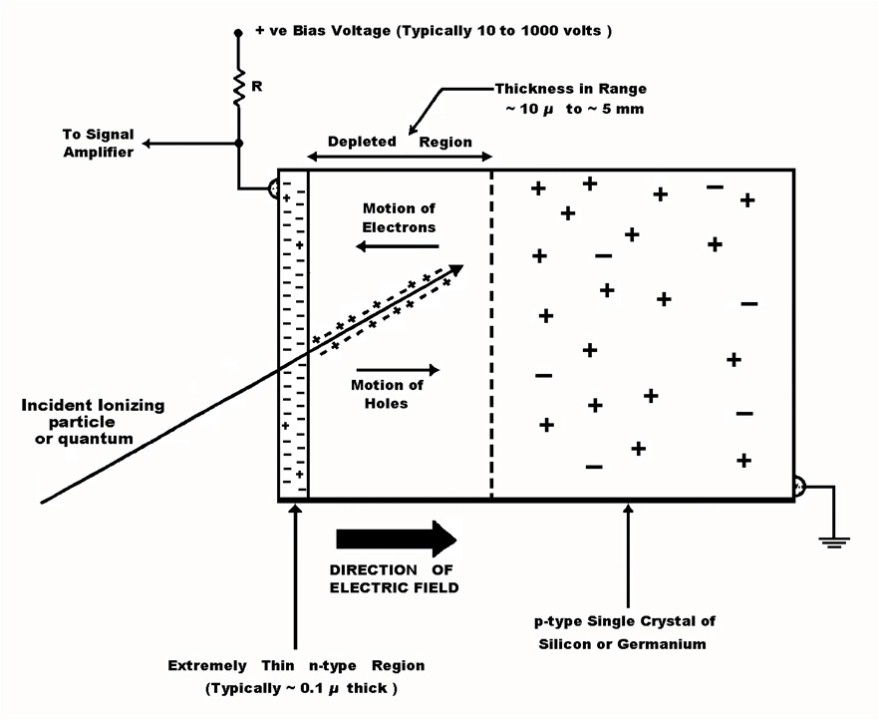
\includegraphics[scale=0.35]{ch9/image1}
	\captionof{figure}{ }
	\end{wrapfigure}
	
Un rayonnement traversant la zone de déplétion d'une jonction $pn$ polarisée en inverse crée de
nombreuses paires électron-trou. Les électrons vont aller vers le pôle positif et les trous vers
le pôle négatif : comme dans la chambre d'ionisation, il va apparaître un courant. Il s'agit donc
ici d'une chambre ionisation mais de taille bien plus réduite.\\

Le nombre de paires est étant directement proportionnelle à l'énergie cédée, l'intensité du courant 
(et donc l'impulsion de tension aux bornes d'une résistance) est directement proportionnelle à cette
énergie. Ce détecteur permet ainsi à la fois le comptage et la spectrométrie.

\subsection{Collecte des charges}%sl28
	\begin{wrapfigure}[5]{r}{4cm}
	\vspace{-5mm}
	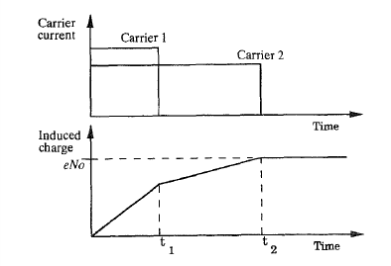
\includegraphics[scale=0.35]{ch9/image2}
	\captionof{figure}{ }
	\end{wrapfigure}
Le dépôt de l'énergie d'un rayonnement ionisant crée un nombre égal d'électrons et de trous. A cause
du champ électrique, ceux-ci vont migrer et former un courant persistant jusqu'au moment où les 
porteurs sont collectés à la frontière du volume actif\footnote{Le signal apparaît encore une fois
directement après la création de la paire.}. La seule différence dans la collecte par 
rapport à une chambre d'ionisation gazeuse est l'échelle de temps. La mobilité des électrons est plus
grande que celle des trous, mais seulement d'un facteur 2-3. On considèrera que les temps de 
collections sont égaux. Le courant total inclut ainsi les courants dus aux \textbf{deux} types de
porteurs.

\section{Détecteurs au silicium}%sl30
L'avantage du Si est que l'on peut l'utiliser à température ambiante. A cette température, 
l'énergie moyenne pour la création d'une paire $e^-/h^+$ est de 3.62 eV. Le désavantage du Si 
est que sa zone de déplétion est de petite taille ($\approx 5$ mm) : on l'utilisera principalement
pour des particules chargées(le libre parcours moyen des $\gamma$ est trop important). On peut 
également l'utiliser pour détecter les trajectoires des particules chargées. La résolution 
typique ($F\approx0.11$) est de 3.5 keV.

\subsection{Diode à jonction diffusée}
Il s'agit de la première jonction utilisé pour la détection. On considère un cristal homogène de
type $p$ et on fait diffuser à haute température une impureté de type donneur pour avoir une zone 
proche de la surface en type $n$. Il en résulte une diode très robuste à surface fortement dopée
causant une forte extensionde la zone de déplétion du côté $p$ jusqu'à formé une zone morte 
équivalente à la zone de diffusion, ce qui est gênant pour les particules charges: plus utilisé.



\subsection{Jonction à barrière de surface}
Il s'agit du type de détecteur au Si le plus utilisé, dont la jonction est formée entre un SC 
et un métal. La différence entre les deux niveau de 
Fermi modifie les bandes du SC et il se forme une barrière de \textsc{Shottky}. La zone de
charge d'espace peut atteindre 5 mm. La fabrication est simple et la zone morte de faible
épaisseur (épaisseur du métal, $\approx$ 20nm), mais il est très sensible à la lumière et fragile
("\textit{Vous la touchez, c'est fini}"). Il se forme également une couche d'oxyde à l'interface. Il
semblerait qu'elle ai une grande importance, mais on ne sait pas pourquoi. Comme ça fonctionne, on se
casse pas plus la tête que ça.\\

\subsubsection{Barrière de Shottky}
	\begin{wrapfigure}[14]{l}{5cm}
	\vspace{-5mm}
	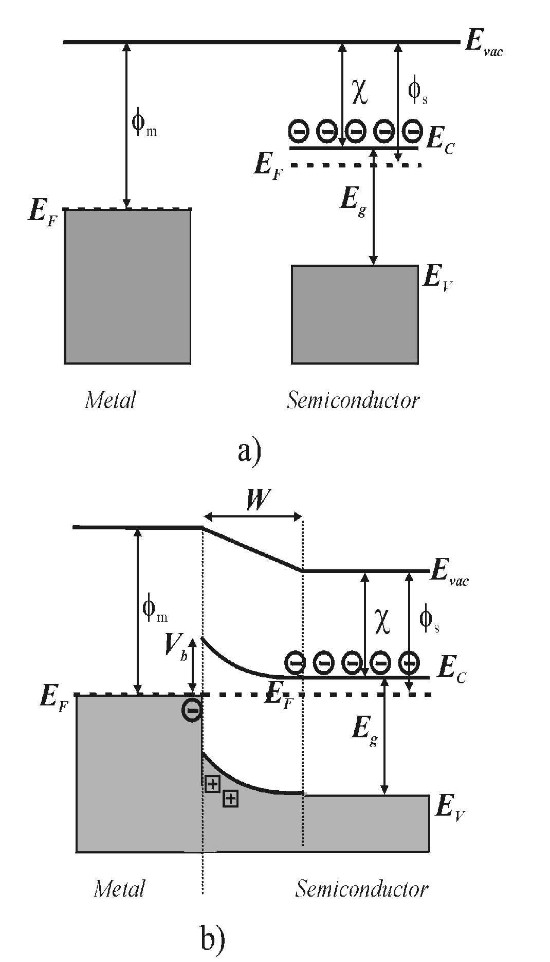
\includegraphics[scale=0.27]{ch9/image3}
	\captionof{figure}{ }
	\end{wrapfigure}
Il ne s'agit pas exactement d'une jonction $pn$ mais le fonctionnement est très similaire. 
Lorsque l'on établit la jonction entre le métal et le SC, les électrons du SC diffusent vers
le métal et une zone du SC se vide d'électron. Cette région contient des charges positives et
il apparaît un champ électrique stoppant la diffusion des électrons. La région de déplétion est
ainsi équivalente à celle d'un contact PN. Deux différences : potentiel de contact plus faible
(on peut prendre aussi fin que l'on veut pour avoir une zone morte très très mince) et région
de déplétion qui s'étend uniquement dans le SC.

\subsection{Jonction par implantation ionique}
On bombarde la surface du SC (type $n$ ou $p$) par un faisceau d'ions donneurs ou accepteurs 
pour injecter les dopants dans le SC. En ajustant le faisceau, on peut contrôler la 
profondeur et la concentration d'impuretés ainsi que le profil. Le contrôle étant parfait,le 
détecteur est très stable et la zone morte très mince, il s'agit du meilleur détecteur actuel 
(très utilisé en physique des hautes énergies). Par contre, il coûte bonbon (il faut avoir un
accélérateurs d'ion pour faire ce type de diode).

\subsection{Jonction compensée au lithium – Si(Li) – Diode p-i-n}
	\begin{wrapfigure}[10]{l}{3cm}
	\vspace{-5mm}
	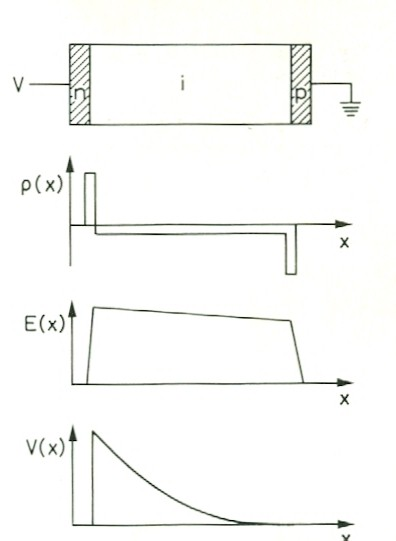
\includegraphics[scale=0.27]{ch9/image4}
	\captionof{figure}{ }
	\end{wrapfigure}
	
Pour augmenter la taille de la zone de déplétion, on utilise un matériau compensé (i) pris en
sandwich entre deux couches de type $p$ et $n$ pour avoir du p-i-n. On dit qu'il s'agit d'un
SC compensé car les impuretés d'un type donné peuvent être compensées par injection d'impuretés
d'un autre type pour avoir la même concentration de donneurs que d'accepteurs. On retrouve alors
les caractéristiques d'un matériau intrinsèque avec en particulier par de charge d'espace dans la
région i.\\

Comme il n'y a pas de charge d'espace, le champ électrique est presque constant et la zone de compensation (zone dans laquelle la particule doit déposer son énergie) peut atteindre une épaisseur de 15mm. On peut détecter des $\beta$ et rayons $X$ de faible énergie.\\

Pour le faire, on considère du Si de type $p$ et on fait diffuser du lithium (donneur) qui 
compense les accepteurs pour faire un détecteur Si(Li). Le Li est utilisé car il a un très
haut coefficient de diffusion lui permettant de se glisser dans les interstices pour former
des paires avec les impuretés de type $p$ du matériau. Le souci est qu'à haute température le Li
continue de diffuser en envahit tout le cristal, il faut donc refroidir le détecteur à l'aide
d'azote liquide.


\subsection{Détecteur à microstrips}
Détecteur constitué 'un substrat de Si de type $n$ sur lequel une série de micro-bandes de $Si$ de
type $p$ sont implantées à 20 $\mu m$ d'intervalle et reliées à des contacts en aluminium. Le nombre
décharge collectées à un contact donné dépend de la trajectoire de la particule. La résolution
spatiale est de 5$\mu$m.

\section{Détecteurs au germanium}%sl42
Comme le Ge possède un gap en énergie faible ($\approx0.7$ eV), les mesures doivent être effectuées
à basse température pour éviter les courants de fuites dus à l'agitation thermique. A 77K, 
l'énergie moyenne pour une paire $e^-/h^+$ est de 2.96 eV. Grâce à son $Z$ élevé, il a une grande
section efficace pour l'effet photoélectrique et il sera ainsi principalement utilisé pour la
détection/spectro $\gamma$. On ne l'utilise pas pour des particules chargées car il n'a pas 
d'avantage par rapport à ceux en Si. Sa résolution pour des $\gamma$ de 1.33 MeV est de
1.7 keV. Son inconvénient majeur est qu'il est \textbf{très} cher!

\subsection{Jonction compensée au lithium – Ge(Li)}
On crée des détecteurs Ge(Li) en diffusant du lithium dans du Ge. En pratique, l'épaisseur de la
zone compensée est de 15 à 20mm. La diffusion du Li impose le refroidissement constant du 
détecteur (et pas seulement pendant l'utilisation). On l'utilise actuellement peu.

\subsection{Détecteur au Ge intrinsèque - HPGe}
On peut actuellement obtenir des cristaux de haute pureté rendant le cristal quasi intrinsèques
: HPGe signifie \textit{High Purity Germanium}. Les cristaux sont légèrement de type $p$ ou de type $n
$ selon la nature des traces d'impuretés résiduelles. Les jonctions détectrices sont réalisées en 
dopant par implantation ionique une des faces du cristal quasi-intrinsèque qui peut être réalisé dans 
de gros volumes. Ici le refroidissement n'est nécessaire que durant l'utilisation. On l'utilise
fréquemment pour réduire la spectro $\gamma$.





































\section{Autres matériaux}%sl50
A bien lire, du slide 50 a 56.